\documentclass{article}

\usepackage[final,nonatbib]{nips_2016}


\usepackage[utf8]{inputenc} % allow utf-8 input
\usepackage[T1]{fontenc}    % use 8-bit T1 fonts
\usepackage{hyperref}       % hyperlinks
\usepackage{url}            % simple URL typesetting
\usepackage{booktabs}       % professional-quality tables
\usepackage{amsfonts}       % blackboard math symbols
\usepackage{nicefrac}       % compact symbols for 1/2, etc.
\usepackage{microtype}      % microtypography
\usepackage{graphicx}

\usepackage[backend=bibtex]{biblatex}
\bibliography{smallbiblio}
\AtEveryBibitem{%
  \clearlist{language}%
}


\title{Neural networks with differentiable structure}

\author{
Thomas Miconi\\%\thanks{Use footnote for providing further
%    information about author (webpage, alternative
%    address)---\emph{not} for acknowledging funding agencies.} \\
  The Neurosciences Institute\\
 La Jolla, CA, USA \\
  \texttt{miconi@nsi.edu} \\
}

\begin{document}
 
\maketitle

\begin{abstract}

While gradient descent has proven highly successful in learning connection
weights for neural networks, the actual structure of these networks is usually determined by hand, or by
other optimization algorithms.  Here we describe a simple method to make
network structure differentiable, and therefore accessible to gradient descent.
We test this method on recurrent neural networks applied to simple
sequence prediction problems. Starting with initial networks containing only
one node, the method automatically builds networks that successfully solve the
tasks. The number of nodes in the final network correlates with task
difficulty. The method can dynamically increase network size in response to an
abrupt complexification in the task; however, reduction in network size in
response to task simplification is not evident for meta-parameters used here.
The method does not penalize network performance for these test tasks:
variable-size networks actually reach better performance than fixed-size
networks of higher, lower or identical size. We conclude by discussing how this
method could be applied to more complex networks, such as feedforward layered
networks, or multiple-area networks of arbitrary shape.

\end{abstract}

\section{Introduction}

Neural networks are usually optimized by applying some form gradient descent to
the numerical parameters of a fixed connectivity graph. This method can
successfully train very large networks for complex tasks. However, the actual
structure of the network itself (number of neurons, connectivity graph, etc.) is usually not modified by the gradient
descent algorithm. Most often, network structure is designed by hand, in a delicate process of parameter tuning.
When network structure is optimized, it is generally with a different
algorithm, including evolutionary techniques such as NEAT \cite{Stanley2002-ug} or heuristic-based methods such as HyperOpt \cite{Yamins2014-us}.

Manual design of network structure is time-consuming and subject to arbitrary
choices that may or may not reflect the demands of the task at hand. It would
therefore be desirable to extend the process of gradient descent to network
structure itself. This requires making network structure differentiable, at
least to a usable approximation. Here we describe a simple method
for performing gradient descent over network structure, and show that this
method can adaptively design recurrent networks of a few dozen units for simple
sequence prediction
tasks.


\section{Method}

\subsection{Description of the algorithm}

Here we describe our method, in the context of recurrent networks with
all-to-all potential connectivity (in the conclusion, we suggest how the method
could be extended to more complex architectures, including layered feedforward
networks). In this situation, structure is determined by the number of nodes in
the network $N$, which automatically determines the connectivity graph as a
simple square matrix of size $N*N$. Our goal is to make the number of nodes
differentiable and amenable to gradient descent and backpropagation. 

The first step in our method is to apply a scalar \textit{multiplier} to
the output of every node in the network. These multipliers are part of the
network graph and undergo backpropagation of error gradients,
just like other parameters of the network; however, they also undergo a strong
regularization based on minimizing the L1-norm (i.e. the sum of absolute
values) of all multipliers. 

Minimizing the L1-norm does not just minimize the value of the multipliers, but
also tends to concentrate the remaining total weight among the fewest possible
elements, in comparison to Euclidean L2-norm minimization.  As a result,
backpropagation will tend to minimize the number of non-zero multipliers, and
thus of ``active'' neurons: each neuron must ``earn its keep'', by contributing
to overall network performance, to counter-balance the effect of L1-norm
minimization, or else face effective ``soft'' deletion by having its multiplier
set to zero.\footnote{Importantly, note that L1 regularization on multipliers
    applied to neuron activities is quite different from directly imposing an
    L1 regularization on neuron activities themselves. L1 regularization of
    neuron activities ensures that few neurons will be active \textit{at any
    given time}, but does not ensure that any neuron will become fully silent
    over extended time.  Instead, L1 regularization of neuron activities may
    encourage neurons to distribute and decorrelate their activations other
    time so that each neuron responds to a small proportion of inputs; this is
    precisely the (intended) effect of L1-regularization in \textit{sparse
coding} schemes \cite{Olshausen1996-vz}. By contrast, multipliers can truly
turn neurons ``on'' or ``off'' in a time-independent fashion: a neuron with a
zero multiplier is guaranteed to be silent for any input. }

Applying L1-regularized, error-backpropagated multipliers to neuron outputs creates a ``soft''
structural variability, whereby gradient descent tries to solve the task at
hand under the constraint of minimizing the number of neurons with a non-zero
multiplier. We want to turn these ``soft'' structure changes into hard
structural changes in the actual number of neurons and size of the weight
matrix. To this end, we first specify a \textit{deletion threshold} $T_D$, such
that any node whose multiplier falls below this threshold is marked for
potential deletion. Then, we simply specify that at any given time, the network
must only contain a fixed, small number $k$ of neurons below the deletion
threshold. If the number of sub-threshold neurons exceeds $k$, then ``excess''
sub-threshold neurons are actually deleted from the network.  Conversely, if
backpropagation finds it necessary to inflate multipliers to the extent that
fewer than $k$ neurons have sub-threshold multipliers, then we add a new neuron
to the simulation, with initially random connectivity and a multiplier
initially set exactly at the threshold value. Note that, because the threshold
value is low, new neurons initially have a very small effect on overall network
behavior.

This mechanism allows backpropagation to adjust network size to problem
demands. If more neurons are needed to solve the problem at hand,
backpropagation will simply expand the multipliers of currently sub-threshold
neurons, so as to allow them to have an impact on output computation, while adjusting their connectivity. By
contrast, if new neurons fail to contribute to network performance,
L1-minimization  will reduce their multipliers and eventually drive them below
deletion threshold. The sub-threshold neurons thus act as a computational
reserve, ready to be mobilized if the problem at hand demands it.

Note that multipliers can be  applied either as an intermediate layer of
weights between hidden and output neurons (thus affecting only the input to
output neurons), or directly to the output of hidden neurons (thus affecting
both feedforward and recurrent inputs). Our experiments confirm that both methods work; however, somewhat surprisingly, the 
former method produces noticeably better performance. 
Thus, for all results reported in this paper, we apply multipliers only to the output of hidden neurons that is fed to the output neurons,
leaving recurrent hidden-to-hidden inputs unaffected by the multipliers. 


Finally, as a stabilization measure, we make
addition and deletion probabilistic, so that whenever a neuron is to be added
or deleted, the event only occur with a certain fixed probability $P_{add}$ or
$P_{del}$. As a result, the network will occasionally possess more or less than
$k$ subthreshold neurons. All networks in our experiment start with only one
node, following the philosophy of ``augmenting topologies'' expounded in NEAT
\cite{Stanley2002-ug}.

\subsection{Implementation details}

Our implementation is based on Andrej Karpathy's \verb+min-char-rnn.py+ and
inherits most of its parameters.  The networks are trained for 300000 cycles,
where each cycle consists of reading a sequence of 40 characters while trying
to predict the next character, followed by a parameter update based on
backpropagation through time. Network output is provided by a single output
layer with 4 nodes (one per possible character), each of which reports the
predicted probability that the corresponding character is next in the sequence. The output layer is fully connected with the variable-size recurrent layer.
Loss is defined as cross-entropy between the predicted distribution and the
actual (one-hot) outcome. Multipliers are updated similarly to other network
parameters. Any addition or deletion also occurs at the same time as parameter
update (that is, at the end of each successive 40-char sequence). 

All multipliers are bounded from below by a low, but not trivial
value $M_{min}$. If a parameter update drives the value of a multiplier below $M_{min}$, it is automatically set to $M_{min}$. The intended effect is that every neuron (even those with multipliers
below deletion threshold) should still have a small, but not negligible effect
on network output, so that a reasonable gradient of error over any neuron's
parameters can always be computed. This allows all neurons to always be ``ready to help'' if needed. An additional side-effect is to make all multipliers strictly positive, although this is not a critical component of our method.


There are thus 6 additional parameters in our method: $k$, $T_D$, $M_{min}$, $P_{add}$,
$P_{del}$, and $A_{L1reg}$ (the strength of the L1 regularization
over the multipliers). In all simulations shown here, those were set to $k=1$,
$T_D=0.05$,  $M_{min}=0.025$, $P_{add}=0.05$, $P_{del}=0.25$, and
$A_{L1reg}=3*10^{-5}$. 


All code is available on GitHub at \url{https://github.com/ThomasMiconi/DiffRNN}.


\section{Experiments}

\subsection{Tasks}

To test the plausibility of our method, we choose two simple sequence prediction
problems. In each problem, the task of the network is to predict the next
character in an ongoing sequence of characters. Both problems use the same
alphabet, consisting of characters $a$, $b$, $($ and $)$. 

The first problem (``easy problem'') is composed of groups of one or more $ab$
digraphs, enclosed in matching parentheses. After every $ab$ digraph, there is
a constant probability of adding an additional $ab$ digraph, or to close the
group with a closing parenthesis instead. Thus the number of digraphs in each
group follows an exponential distribution. A typical sequence looks like this:

\begin{center}
$(abab)(ab)(ab)(ababab)(ab)(abab)(abababab)\ldots$
\end{center}

Note that the problem is highly constrained: the only choice occurs after a
$b$, when the network must decide whether to insert a $)$ or an $a$, which has
a well-defined probability. Every other choice is unambiguously specified by the problem. 


The second problem (''hard problem'') is composed of groups of five letters
enclosed in matching parentheses. The rule is that each new group must be the
reverse of the previous group, with one randomly chosen letter changed. A
typical sequence looks like this:

\begin{center}
$(abbab)(babaa)(aabbb)(bbaaa)(baabb)(baaab) \ldots$
\end{center}

To reach optimal performance on this task, the network must maintain a memory
of the previous sequence of five characters, and then reverse it. This is a
much more difficult problem than the previous one, and thus we expect that
optimal networks for either task would look quite different from each other.

\section{Results}

\begin{figure}[ht]
\label{fig:easyandhard}
  \centering
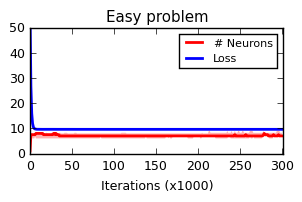
\includegraphics[scale=0.9]{figE.png}
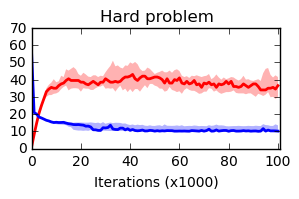
\includegraphics[scale=0.9]{figH.png}
  \caption{Model performance on an easy task (left panel) and a hard task
(right panel). Both performance (cross-entropy loss between predicted and
actual character) and number of neurons are shown as a function of time. Dark curves and shaded areas indicate median and inter-quartile range over 20 runs, respectively. The
model settles on larger network size for the more complex problem. }
\end{figure}


\subsection{Performance and network size in hard and easy tasks}


Results are shown in Figure \ref{fig:easyandhard}. We show both median
performance (cross-entropy loss) and median number of neurons as a function of
time, over 20 runs. As expected, the hard problem leads to somewhat higher loss
than the easy problem. Importantly, the hard problem elicits larger networks
than the easy problem (27 neurons vs. 6 neurons after 300000 learning cycles).
Thus, the algorithm appropriately allocated more neurons to solve a more difficult
task.

An important question is whether the use of variable-size networks has an
impact on performance. We compared the performance of our algorithm against
fixed-size networks with various numbers of neurons, ranging from 10 to 100,
including one with the same network size as was eventually preferred by our
algorithm (i.e. 27 neurons).  Results are shown in figure \ref{fig:fixedsize},
again showing the median loss among 20 runs as a function of time. First, note
that performance is not a simple function of network size: the
best-performing fixed-size network is actually the one with 27 neurons, while
100 neurons 
produces the poorest performance.

Intriguingly, the variable-size network actually outperforms fixed-size
networks of any size.  This result should not be over-interpreted: the
variable-size program contains additional meta-parameters, which were
themselves manually adjusted by experimentation, making the comparison somewhat
unfair. However, this result suggests that adding network size to the learning
process do not necessarily lead to worse performance. 


\subsection{Dynamical adjustment of network size in response to changing conditions}

What happens if task difficulty suddenly changes? We tested our network by
 switching from the ``easy'' to the ``hard'' sequence after 100000
cycles, and then back again to the ``easy'' sequence after 200000 cycles.
Results are shown in Figure \ref{fig:easyhardeasy}. Interestingly, the network
successfully handles the abrupt complexification of the problem by allocating
more neurons. However, when the problem switches back to the ``easy'' sequence,
performance quickly returns to optimal levels, but the network remains large.
Thus, the algorithm can increase network size in response to problem
complexification, but does not reduce network size much in response to problem
simplification.


\begin{figure}[t]
\label{fig:fixedsize}
  \centering
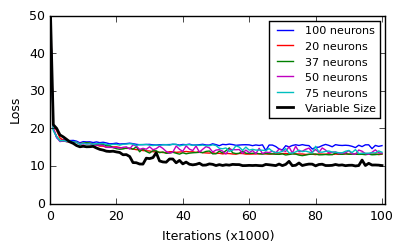
\includegraphics[scale=0.9]{figFS.png}
  \caption{Comparison of performance for variable and fixed size, for the
``hard'' problem. The thick black line shows variable-size network performance
and is identical to the blue curve in Fig. \ref{fig:easyandhard}, right panel.
Thin colored curves indicate performance of fixed-size networks of various
sizes. Curves show medians over 20
runs; inter-quartile ranges (not shown for clarity) are comparable to those
seen in Fig. \ref{fig:easyandhard}. Notice that performance is not a simple
function of network size. Variable-size networks seem to outperform fixed-size
networks, though this should be interpreted with caution (see text). }
\end{figure}

\begin{figure}[b]
\label{fig:easyhardeasy}
  \centering
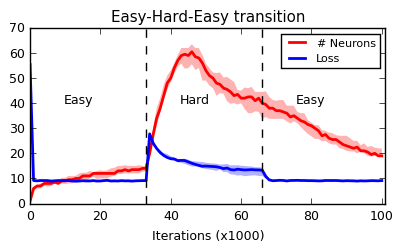
\includegraphics[scale=0.9]{figEHE.png}
  \caption{Dynamic adjustment of network size in response to abrupt complexification, but not simplification, of an ongoing task.}
\end{figure}



Anecdotally, we found that it was possible to adjust parameters so that network
size would be reduced in response to problem simplification; however this
parameter regime leads to noticeably worse performance on the ``hard''
problem. This may reflect a trade-off between adaptability and performance,
in which the algorithm is reluctant to adjust network size once optimal
performance is reached (which occurs quickly after the hard-to-easy
transition). More work is needed to elucidate the conditions that allow or
restrict network size adjustment.


\section{Conclusions and future work}

We have described a method through which the size of a recurrent network can be
modified by gradient descent. The method described here can successfully build
networks of appropriate size to handle simple problems. This simple method
immediately suggests several alternatives and possible extensions.

For example, deletion of neurons could be biased by neuron ``age'' (i.e. how
long the neuron has been present), rather than being random. Deleted neurons
could be partially preserved, so that newly added neurons could actually
inherit connectivity of previously deleted ones, rather than being randomly
initialized. Such adaptations were not necessary for the problems considered
here, but might be considered in future applications to more challenging tasks.

The method described here extends naturally to layered feedforward networks.
Within each layer, the method can be applied essentially unchanged to adjust
layer size. The number of layers can also be made differentiable, by adding and deleting
residual layers \cite{He2015-gk} with initially low multipliers on their
pre-additive output. These residual layers, which would initially have minimal impact
on the network's output, would play the same role as sub-threshold neurons in
the method described above.


A more distant goal would be to  apply differentiability to network
interactions - for example, whether the output of a given node should have an
additive or multiplicative (modulatory) effect on its targets. In theory, this
might be done by maintaining two links between any two connected neurons (one
additive and one multiplicative), and applying a gradient-descendable ratio
between the two.  Similarly, by considering each layer as a higher-order
``node'', subject to a global multiplier, the method described above could in
principle be extended to arbitrary networks composed of multiple areas, with
arbitrary connectivity between areas. Further work is needed to assess the
practicality of these and other possible extensions.


\small

\printbibliography

\end{document}
